\documentclass{standalone}
\usepackage{tikz}
\begin{document}
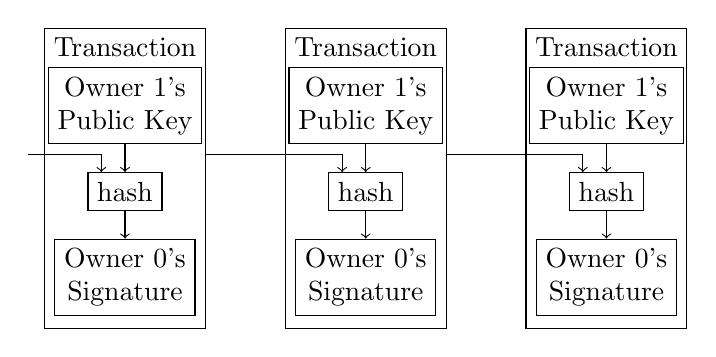
\begin{tikzpicture}
	\node (trans1) [draw, text depth = 9.5em] {Transaction};
	\node (pub1) [draw, align=center, anchor = north] at ([yshift=-5mm] trans1.north) {Owner 1's\\Public Key};%
	\node (hash1) [draw, anchor = north] at ([yshift = -1em] pub1.south) {hash};%
	\node (sig0) [draw, align=center, anchor = north] at ([yshift=-1em] hash1.south) {Owner 0's\\Signature};%

	\node (trans2) [draw, text depth = 9.5em, anchor = west] at ([xshift = 1cm] trans1.east){Transaction};
	\node (pub2) [draw, align=center, anchor = north] at ([yshift=-5mm] trans2.north) {Owner 1's\\Public Key};%
	\node (hash2) [draw, anchor = north] at ([yshift = -1em] pub2.south) {hash};%
	\node (sig1) [draw, align=center, anchor = north] at ([yshift=-1em] hash2.south) {Owner 0's\\Signature};%

	\node (trans3) [draw, text depth = 9.5em, anchor = west] at ([xshift = 1cm] trans2.east){Transaction};
	\node (pub3) [draw, align=center, anchor = north] at ([yshift=-5mm] trans3.north) {Owner 1's\\Public Key};%
	\node (hash3) [draw, anchor = north] at ([yshift = -1em] pub3.south) {hash};%
	\node (sig2) [draw, align=center, anchor = north] at ([yshift=-1em] hash3.south) {Owner 0's\\Signature};%

	\draw[->] (pub1) -- (hash1);
	\draw[->] (pub2) -- (hash2);
	\draw[->] (pub3) -- (hash3);

	\draw[->] (hash1) -- (sig0);
	\draw[->] (hash2) -- (sig1);
	\draw[->] (hash3) -- (sig2);

	\draw[->] ([yshift = 3mm, xshift = -2mm] trans1.west) -| ([xshift = -3mm] hash1.north);
	\draw[->] ([yshift = 3mm] trans1.east) -| ([xshift = -3mm] hash2.north);
	\draw[->] ([yshift = 3mm] trans2.east) -| ([xshift = -3mm] hash3.north);
\end{tikzpicture}
\end{document}
